% Day 12: MLflow Basics - Complete Guide
% Databricks-themed LaTeX Beamer Presentation
\documentclass[aspectratio=169]{beamer}

% ============================================
% PACKAGES
% ============================================
\usepackage{tikz}
\usepackage{graphicx}
\usepackage{hyperref}
\usepackage{xcolor}
\usepackage{listings}
\usepackage{fontawesome5}
\usepackage{booktabs}
\usepackage{array}
\usepackage{colortbl}
\usepackage{amsmath}
\usetikzlibrary{shapes.geometric, arrows.meta, positioning, calc, shadows, decorations.pathreplacing}

% ============================================
% DATABRICKS COLOR PALETTE
% ============================================
\definecolor{databricksBlue}{RGB}{41, 49, 66}
\definecolor{databricksRed}{RGB}{220, 53, 69}
\definecolor{databricksYellow}{RGB}{255, 193, 7}
\definecolor{databricksGreen}{RGB}{76, 175, 80}
\definecolor{databricksGray}{RGB}{128, 128, 128}
\definecolor{databricksLightGray}{RGB}{245, 245, 245}
\definecolor{databricksWhite}{RGB}{255, 255, 255}
\definecolor{codeBackground}{RGB}{40, 44, 52}
\definecolor{databricksOrange}{RGB}{255, 140, 0}

% ============================================
% BEAMER THEME CONFIGURATION
% ============================================
\usetheme{default}
\usecolortheme{default}

% Set colors
\setbeamercolor{structure}{fg=databricksBlue}
\setbeamercolor{title}{fg=databricksWhite}
\setbeamercolor{frametitle}{fg=databricksWhite,bg=databricksBlue}
\setbeamercolor{normal text}{fg=databricksBlue}
\setbeamercolor{block title}{fg=databricksWhite,bg=databricksBlue}
\setbeamercolor{block body}{fg=databricksBlue,bg=databricksLightGray}
\setbeamercolor{itemize item}{fg=databricksBlue}
\setbeamercolor{itemize subitem}{fg=databricksRed}
\setbeamercolor{itemize subsubitem}{fg=databricksGreen}
\setbeamercolor{footline}{fg=databricksWhite,bg=databricksBlue}

% Remove navigation symbols
\setbeamertemplate{navigation symbols}{}

% Bullet point styles
\setbeamertemplate{itemize item}{\textcolor{databricksBlue}{$\bullet$}}
\setbeamertemplate{itemize subitem}{\textcolor{databricksRed}{$\triangleright$}}
\setbeamertemplate{itemize subsubitem}{\textcolor{databricksGreen}{$\circ$}}

% ============================================
% FOOTER CONFIGURATION
% ============================================
\setbeamertemplate{footline}{%
  \leavevmode%
  \hbox{%
    \begin{beamercolorbox}[wd=.30\paperwidth,ht=2.5ex,dp=1ex,left]{footline}%
      \hspace*{2ex}\href{https://easy-ai-labs.lovable.app/}{\textcolor{databricksWhite}{\footnotesize Easy AI Labs}}
    \end{beamercolorbox}%
    \begin{beamercolorbox}[wd=.40\paperwidth,ht=2.5ex,dp=1ex,center]{footline}%
      \href{https://www.linkedin.com/in/yashkavaiya}{\textcolor{databricksWhite}{\footnotesize Yash Kavaiya}}
    \end{beamercolorbox}%
    \begin{beamercolorbox}[wd=.20\paperwidth,ht=2.5ex,dp=1ex,center]{footline}%
      \href{https://www.linkedin.com/company/genai-guru}{\textcolor{databricksWhite}{\footnotesize Gen AI Guru}}
    \end{beamercolorbox}%
    \begin{beamercolorbox}[wd=.10\paperwidth,ht=2.5ex,dp=1ex,right]{footline}%
      \textcolor{databricksWhite}{\footnotesize \insertframenumber/\inserttotalframenumber}\hspace*{2ex}
    \end{beamercolorbox}%
  }%
  \vskip0pt%
}

% ============================================
% CODE LISTING STYLE
% ============================================
\lstdefinestyle{databrickscode}{
    backgroundcolor=\color{codeBackground},
    basicstyle=\ttfamily\scriptsize\color{databricksWhite},
    keywordstyle=\color{databricksYellow}\bfseries,
    stringstyle=\color{databricksGreen},
    commentstyle=\color{databricksGray}\itshape,
    breaklines=true,
    frame=single,
    rulecolor=\color{databricksBlue},
    showstringspaces=false,
    numbers=none,
    xleftmargin=2pt,
    xrightmargin=2pt,
    aboveskip=8pt,
    belowskip=8pt
}
\lstset{style=databrickscode}

% ============================================
% TITLE PAGE INFO
% ============================================
\title{\textbf{Day 12: MLflow Basics}}
\subtitle{Complete Guide to ML Lifecycle Management}
\author{Databricks 14-Days AI Challenge}
\date{\today}
\institute{MLflow - Tracking - Model Registry - Deployment}

% ============================================
% CUSTOM TITLE PAGE
% ============================================
\setbeamertemplate{title page}{
    \begin{tikzpicture}[remember picture, overlay]
        \fill[databricksBlue] (current page.north west) rectangle (current page.south east);
        
        % Title
        \node[anchor=center, text=databricksWhite, font=\Huge\bfseries] 
            at ([yshift=1.5cm]current page.center) {\inserttitle};
        
        % Subtitle
        \node[anchor=center, text=databricksYellow, font=\Large] 
            at ([yshift=0.3cm]current page.center) {\insertsubtitle};
        
        % Author
        \node[anchor=center, text=databricksWhite, font=\large] 
            at ([yshift=-1cm]current page.center) {\insertauthor};
        
        % Institute
        \node[anchor=center, text=databricksGray, font=\normalsize] 
            at ([yshift=-2cm]current page.center) {\insertinstitute};
        
        % Decorative elements
        \node[anchor=center, text=databricksRed, font=\fontsize{60}{60}\selectfont, opacity=0.3] 
            at ([xshift=-5cm, yshift=2.5cm]current page.center) {\faFlask};
        \node[anchor=center, text=databricksGreen, font=\fontsize{50}{50}\selectfont, opacity=0.3] 
            at ([xshift=5cm, yshift=-1cm]current page.center) {\faChartLine};
    \end{tikzpicture}
}

% ============================================
% DOCUMENT BEGIN
% ============================================
\begin{document}

% Title Slide
\begin{frame}[plain]
    \titlepage
\end{frame}

% ============================================
% TABLE OF CONTENTS
% ============================================
\begin{frame}{Agenda}
    \begin{columns}[T]
        \begin{column}{0.5\textwidth}
            \begin{itemize}
                \item \textcolor{databricksBlue}{\textbf{Introduction to MLflow}}
                \item \textcolor{databricksBlue}{\textbf{MLflow Components}}
                \item \textcolor{databricksBlue}{\textbf{MLflow Tracking}}
                \item \textcolor{databricksBlue}{\textbf{Model Registry}}
                \item \textcolor{databricksBlue}{\textbf{MLflow Models}}
                \item \textcolor{databricksBlue}{\textbf{Experiment Tracking}}
            \end{itemize}
        \end{column}
        \begin{column}{0.5\textwidth}
            \begin{itemize}
                \item \textcolor{databricksBlue}{\textbf{Model Logging}}
                \item \textcolor{databricksBlue}{\textbf{MLflow UI}}
                \item \textcolor{databricksBlue}{\textbf{Practical Implementation}}
                \item \textcolor{databricksBlue}{\textbf{Comparing Runs}}
                \item \textcolor{databricksBlue}{\textbf{Best Practices}}
            \end{itemize}
        \end{column}
    \end{columns}
\end{frame}

% ============================================
% SECTION: INTRODUCTION TO MLFLOW
% ============================================
\begin{frame}{What is MLflow?}
    \begin{block}{Definition}
        MLflow is an \textcolor{databricksRed}{\textbf{open-source platform}} designed to manage the complete machine learning lifecycle.
    \end{block}
    
    \vspace{0.3cm}
    
    \begin{columns}[T]
        \begin{column}{0.5\textwidth}
            \textcolor{databricksBlue}{\textbf{Key Challenges Solved:}}
            \begin{itemize}
                \item \textcolor{databricksRed}{$\triangleright$} Reproducibility issues
                \item \textcolor{databricksRed}{$\triangleright$} Experiment management
                \item \textcolor{databricksRed}{$\triangleright$} Model versioning
                \item \textcolor{databricksRed}{$\triangleright$} Deployment complexity
                \item \textcolor{databricksRed}{$\triangleright$} Team collaboration
            \end{itemize}
        \end{column}
        \begin{column}{0.5\textwidth}
            \textcolor{databricksBlue}{\textbf{How MLflow Helps:}}
            \begin{itemize}
                \item \textcolor{databricksGreen}{$\circ$} Tracks all parameters and versions
                \item \textcolor{databricksGreen}{$\circ$} Centralized experiment history
                \item \textcolor{databricksGreen}{$\circ$} Model Registry for versioning
                \item \textcolor{databricksGreen}{$\circ$} Unified deployment format
                \item \textcolor{databricksGreen}{$\circ$} Shared tracking server and UI
            \end{itemize}
        \end{column}
    \end{columns}
\end{frame}

% ============================================
% MLFLOW ARCHITECTURE
% ============================================
\begin{frame}{MLflow Architecture Overview}
    \begin{center}
        \begin{tikzpicture}[
            box/.style={rectangle, rounded corners, draw=databricksBlue, fill=databricksLightGray, 
                        text=databricksBlue, minimum width=2.5cm, minimum height=1cm, 
                        font=\footnotesize, align=center, thick},
            arrow/.style={-{Stealth[scale=1.2]}, thick, databricksGray}
        ]
            % Components
            \node[box, fill=databricksYellow!20] (tracking) at (0,2) {\faChartBar\\ Tracking};
            \node[box, fill=databricksRed!20] (registry) at (3,2) {\faBoxes\\ Registry};
            \node[box, fill=databricksGreen!20] (models) at (6,2) {\faCubes\\ Models};
            \node[box, fill=databricksBlue!20] (projects) at (9,2) {\faFolder\\ Projects};
            
            % Storage
            \node[box] (backend) at (2.5,0) {\faDatabase\\ Backend Store};
            \node[box] (artifact) at (6.5,0) {\faCloud\\ Artifact Store};
            
            % UI
            \node[box, fill=databricksOrange!20] (ui) at (4.5,-1.5) {\faDesktop\\ MLflow UI};
            
            % Data Scientist
            \node[font=\Large, text=databricksBlue] (ds) at (-2.5,2) {\faUserGraduate};
            
            % Arrows
            \draw[arrow] (ds) -- (tracking);
            \draw[arrow] (tracking) -- (backend);
            \draw[arrow] (tracking) -- (artifact);
            \draw[arrow] (tracking) -- (registry);
            \draw[arrow] (registry) -- (models);
            \draw[arrow] (backend) -- (ui);
            \draw[arrow] (artifact) -- (ui);
        \end{tikzpicture}
    \end{center}
\end{frame}

% ============================================
% MLFLOW COMPONENTS
% ============================================
\begin{frame}{MLflow Components Overview}
    \begin{center}
        \scriptsize
        \begin{tabular}{p{2cm}p{3.3cm}p{3.3cm}p{3.3cm}}
            \toprule
            \rowcolor{databricksBlue!20}
            \textbf{Component} & \textbf{Purpose} & \textbf{Key Features} & \textbf{When to Use} \\
            \midrule
            \textcolor{databricksYellow}{\textbf{Tracking}} & Record and query experiments & Log params, metrics, artifacts & During model development \\
            \addlinespace[0.2cm]
            \textcolor{databricksRed}{\textbf{Registry}} & Centralized model store & Versioning, stage transitions & Managing production models \\
            \addlinespace[0.2cm]
            \textcolor{databricksGreen}{\textbf{Models}} & Standard packaging format & Framework-agnostic, deploy options & Deploying to production \\
            \addlinespace[0.2cm]
            \textcolor{databricksBlue}{\textbf{Projects}} & Reproducible runs & Package code with dependencies & Sharing code across envs \\
            \bottomrule
        \end{tabular}
    \end{center}
\end{frame}

% ============================================
% MLFLOW TRACKING
% ============================================
\begin{frame}[fragile]{MLflow Tracking - Core Concepts}
    \begin{block}{What is MLflow Tracking?}
        Component responsible for \textcolor{databricksRed}{\textbf{logging and querying experiments}}
    \end{block}
    
    \vspace{0.2cm}
    
    \begin{columns}[T]
        \begin{column}{0.5\textwidth}
            \textcolor{databricksBlue}{\textbf{What Gets Recorded:}}
            \begin{itemize}
                \item \textcolor{databricksBlue}{\textbf{Parameters:}} Input configurations
                \item \textcolor{databricksBlue}{\textbf{Metrics:}} Performance measurements
                \item \textcolor{databricksBlue}{\textbf{Artifacts:}} Output files (models, plots)
                \item \textcolor{databricksBlue}{\textbf{Source:}} Code version and entry point
                \item \textcolor{databricksBlue}{\textbf{Tags:}} Custom metadata
            \end{itemize}
        \end{column}
        \begin{column}{0.5\textwidth}
            \textcolor{databricksBlue}{\textbf{Experiment Structure:}}
            \begin{lstlisting}[basicstyle=\ttfamily\tiny\color{databricksWhite}]
Experiment: "Customer Churn"
|-- Run 1: Random Forest 
|         (accuracy: 0.85)
|-- Run 2: Logistic Regression 
|         (accuracy: 0.78)
|-- Run 3: XGBoost 
|         (accuracy: 0.89)
            \end{lstlisting}
        \end{column}
    \end{columns}
\end{frame}

% ============================================
% TRACKING API
% ============================================
\begin{frame}[fragile]{MLflow Tracking API}
    \begin{lstlisting}[language=Python]
import mlflow

# Experiment Management
mlflow.set_experiment("my_experiment")      
mlflow.create_experiment("new_experiment")  

# Run Management
mlflow.start_run(run_name="my_run")         
mlflow.end_run()                           

# Logging Functions
mlflow.log_param("param_name", value)       
mlflow.log_params({"p1": v1, "p2": v2})    
mlflow.log_metric("metric_name", value)     
mlflow.log_metrics({"m1": v1, "m2": v2})   
mlflow.log_artifact("path/to/file")         
mlflow.set_tag("tag_name", "value")        
    \end{lstlisting}
\end{frame}

% ============================================
% MODEL REGISTRY
% ============================================
\begin{frame}{MLflow Model Registry}
    \begin{block}{What is the Model Registry?}
        A \textcolor{databricksRed}{\textbf{centralized model store}} providing versioning, stage transitions, lineage tracking, and approval workflows.
    \end{block}
    
    \vspace{0.3cm}
    
    \begin{center}
        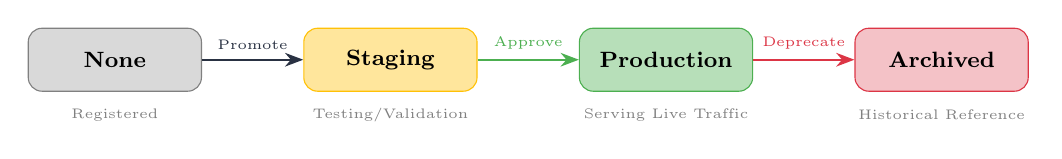
\begin{tikzpicture}[
            stage/.style={rectangle, rounded corners=5pt, minimum width=2.2cm, 
                          minimum height=0.8cm, font=\footnotesize\bfseries, align=center},
            arrow/.style={-{Stealth[scale=1]}, thick}
        ]
            \node[stage, fill=databricksGray!30, draw=databricksGray] (none) at (0,0) {None};
            \node[stage, fill=databricksYellow!40, draw=databricksYellow] (staging) at (3.5,0) {Staging};
            \node[stage, fill=databricksGreen!40, draw=databricksGreen] (prod) at (7,0) {Production};
            \node[stage, fill=databricksRed!30, draw=databricksRed] (archive) at (10.5,0) {Archived};
            
            \draw[arrow, databricksBlue] (none) -- node[above, font=\tiny] {Promote} (staging);
            \draw[arrow, databricksGreen] (staging) -- node[above, font=\tiny] {Approve} (prod);
            \draw[arrow, databricksRed] (prod) -- node[above, font=\tiny] {Deprecate} (archive);
            
            % Labels
            \node[font=\tiny, text=databricksGray] at (0,-0.7) {Registered};
            \node[font=\tiny, text=databricksGray] at (3.5,-0.7) {Testing/Validation};
            \node[font=\tiny, text=databricksGray] at (7,-0.7) {Serving Live Traffic};
            \node[font=\tiny, text=databricksGray] at (10.5,-0.7) {Historical Reference};
        \end{tikzpicture}
    \end{center}
\end{frame}

% ============================================
% REGISTRY OPERATIONS
% ============================================
\begin{frame}[fragile]{Model Registry Operations}
    \begin{lstlisting}[language=Python]
from mlflow import MlflowClient

client = MlflowClient()

# Register a model
model_uri = "runs:/<run_id>/model"
mlflow.register_model(model_uri, "MyModelName")

# Transition model stage
client.transition_model_version_stage(
    name="MyModelName",
    version=1,
    stage="Production"
)

# Add descriptions
client.update_registered_model(
    name="MyModelName",
    description="Customer churn prediction using XGBoost"
)
    \end{lstlisting}
\end{frame}

% ============================================
% MLFLOW MODELS
% ============================================
\begin{frame}[fragile]{MLflow Models - Standard Packaging}
    \begin{columns}[T]
        \begin{column}{0.5\textwidth}
            \textcolor{databricksBlue}{\textbf{Model Flavors:}}
            \begin{itemize}
                \item \texttt{mlflow.sklearn} - Scikit-learn
                \item \texttt{mlflow.pytorch} - PyTorch
                \item \texttt{mlflow.tensorflow} - TensorFlow
                \item \texttt{mlflow.xgboost} - XGBoost
                \item \texttt{mlflow.spark} - Spark MLlib
                \item \texttt{mlflow.pyfunc} - Custom models
                \item \texttt{mlflow.transformers} - Hugging Face
            \end{itemize}
        \end{column}
        \begin{column}{0.5\textwidth}
            \textcolor{databricksBlue}{\textbf{Model Directory Structure:}}
            \begin{lstlisting}[basicstyle=\ttfamily\tiny\color{databricksWhite}]
model/
|-- MLmodel           # Metadata
|-- conda.yaml        # Conda env
|-- requirements.txt  # Dependencies
|-- python_env.yaml   # Python env
|-- model.pkl         # Serialized model
|-- input_example.json
            \end{lstlisting}
        \end{column}
    \end{columns}
\end{frame}

% ============================================
% MODEL DEPLOYMENT
% ============================================
\begin{frame}{Model Deployment Options}
    \begin{center}
        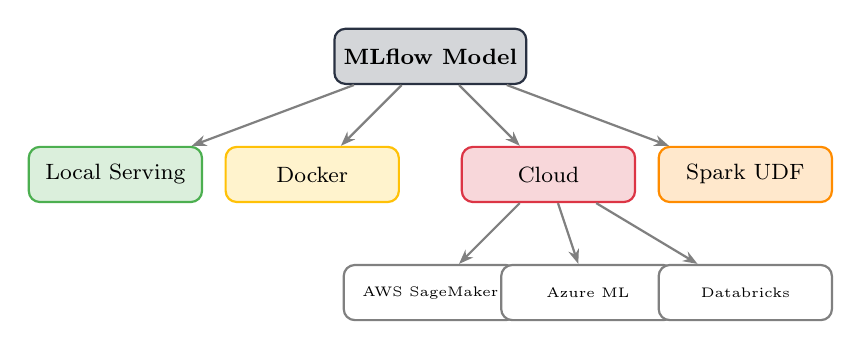
\begin{tikzpicture}[
            box/.style={rectangle, rounded corners, minimum width=2.2cm, minimum height=0.7cm, 
                        font=\footnotesize, align=center, thick},
            arrow/.style={-{Stealth[scale=0.8]}, thick, databricksGray}
        ]
            % Center model
            \node[box, fill=databricksBlue!20, draw=databricksBlue] (model) at (0,0) {\textbf{MLflow Model}};
            
            % Deployment options
            \node[box, fill=databricksGreen!20, draw=databricksGreen] (local) at (-4,-1.5) {Local Serving};
            \node[box, fill=databricksYellow!20, draw=databricksYellow] (docker) at (-1.5,-1.5) {Docker};
            \node[box, fill=databricksRed!20, draw=databricksRed] (cloud) at (1.5,-1.5) {Cloud};
            \node[box, fill=databricksOrange!20, draw=databricksOrange] (spark) at (4,-1.5) {Spark UDF};
            
            % Cloud options
            \node[box, fill=white, draw=databricksGray, font=\tiny] (aws) at (0,-3) {AWS SageMaker};
            \node[box, fill=white, draw=databricksGray, font=\tiny] (azure) at (2,-3) {Azure ML};
            \node[box, fill=white, draw=databricksGray, font=\tiny] (db) at (4,-3) {Databricks};
            
            % Arrows
            \draw[arrow] (model) -- (local);
            \draw[arrow] (model) -- (docker);
            \draw[arrow] (model) -- (cloud);
            \draw[arrow] (model) -- (spark);
            \draw[arrow] (cloud) -- (aws);
            \draw[arrow] (cloud) -- (azure);
            \draw[arrow] (cloud) -- (db);
        \end{tikzpicture}
    \end{center}
\end{frame}

% ============================================
% MODEL URI FORMATS
% ============================================
\begin{frame}{Model URI Formats}
    \begin{center}
        \small
        \begin{tabular}{lll}
            \toprule
            \rowcolor{databricksBlue!20}
            \textbf{URI Format} & \textbf{Description} & \textbf{Example} \\
            \midrule
            \texttt{runs:/<run\_id>/<path>} & Load from specific run & \texttt{runs:/a1b2c3d4/model} \\
            \addlinespace[0.2cm]
            \texttt{models:/<name>/<version>} & Load specific version & \texttt{models:/MyModel/3} \\
            \addlinespace[0.2cm]
            \texttt{models:/<name>/<stage>} & Load from stage & \texttt{models:/MyModel/Production} \\
            \addlinespace[0.2cm]
            \texttt{models:/<name>/latest} & Load latest version & \texttt{models:/MyModel/latest} \\
            \bottomrule
        \end{tabular}
    \end{center}
\end{frame}

% ============================================
% EXPERIMENT TRACKING SETUP
% ============================================
\begin{frame}[fragile]{Experiment Tracking Setup}
    \textcolor{databricksBlue}{\textbf{Three Ways to Configure Tracking:}}
    
    \vspace{0.3cm}
    
    \begin{columns}[T]
        \begin{column}{0.33\textwidth}
            \textcolor{databricksYellow}{\textbf{Local Tracking}}
            \begin{lstlisting}[basicstyle=\ttfamily\tiny\color{databricksWhite}]
import mlflow

# Logs to ./mlruns
mlflow.set_tracking_uri(
    "mlruns"
)
            \end{lstlisting}
        \end{column}
        \begin{column}{0.33\textwidth}
            \textcolor{databricksRed}{\textbf{Remote Server}}
            \begin{lstlisting}[basicstyle=\ttfamily\tiny\color{databricksWhite}]
import mlflow

# Logs to remote
mlflow.set_tracking_uri(
    "http://server:5000"
)
            \end{lstlisting}
        \end{column}
        \begin{column}{0.33\textwidth}
            \textcolor{databricksGreen}{\textbf{Databricks}}
            \begin{lstlisting}[basicstyle=\ttfamily\tiny\color{databricksWhite}]
import mlflow

# Logs to Databricks
mlflow.set_tracking_uri(
    "databricks"
)
            \end{lstlisting}
        \end{column}
    \end{columns}
\end{frame}

% ============================================
% PARAMETERS VS METRICS VS ARTIFACTS
% ============================================
\begin{frame}{Parameters vs Metrics vs Artifacts}
    \begin{center}
        \scriptsize
        \begin{tabular}{p{2cm}p{3.3cm}p{3.3cm}p{3.3cm}}
            \toprule
            \rowcolor{databricksBlue!20}
            \textbf{Aspect} & \textcolor{databricksYellow}{\textbf{Parameters}} & \textcolor{databricksRed}{\textbf{Metrics}} & \textcolor{databricksGreen}{\textbf{Artifacts}} \\
            \midrule
            \textbf{What} & Configuration values & Performance measurements & Files and objects \\
            \addlinespace[0.1cm]
            \textbf{When Set} & Before/during training & During/after training & After computation \\
            \addlinespace[0.1cm]
            \textbf{Data Type} & String (converted) & Numeric & Any file \\
            \addlinespace[0.1cm]
            \textbf{Example} & \texttt{learning\_rate=0.01} & \texttt{accuracy=0.95} & \texttt{model.pkl} \\
            \addlinespace[0.1cm]
            \textbf{Searchable} & Yes & Yes & No (metadata only) \\
            \bottomrule
        \end{tabular}
    \end{center}
\end{frame}

% ============================================
% MODEL LOGGING
% ============================================
\begin{frame}[fragile]{Model Logging - Complete Example}
    \begin{lstlisting}[language=Python, basicstyle=\ttfamily\tiny\color{databricksWhite}]
from mlflow.models.signature import infer_signature

with mlflow.start_run(run_name="complete_example"):
    # Train model
    model = LinearRegression()
    model.fit(X_train, y_train)
    
    # Create signature
    signature = infer_signature(X_train, model.predict(X_train))
    
    # Log model with all options
    mlflow.sklearn.log_model(
        sk_model=model,
        artifact_path="model",
        signature=signature,
        input_example=X_train.iloc[:3],
        registered_model_name="PurchasePredictionModel",
        pip_requirements=["scikit-learn==1.0.2"],
        metadata={"author": "data-team"}
    )
    \end{lstlisting}
\end{frame}

% ============================================
% LOADING MODELS
% ============================================
\begin{frame}[fragile]{Loading Logged Models}
    \begin{lstlisting}[language=Python]
# Method 1: Load from run
model_uri = f"runs:/{run_id}/model"
loaded_model = mlflow.sklearn.load_model(model_uri)

# Method 2: Load from registry
model_uri = "models:/PurchasePredictionModel/Production"
loaded_model = mlflow.sklearn.load_model(model_uri)

# Method 3: Load as generic Python function
loaded_model = mlflow.pyfunc.load_model(model_uri)
predictions = loaded_model.predict(X_test)
    \end{lstlisting}
\end{frame}

% ============================================
% MLFLOW UI
% ============================================
\begin{frame}[fragile]{MLflow UI}
    \begin{columns}[T]
        \begin{column}{0.5\textwidth}
            \textcolor{databricksBlue}{\textbf{Starting the UI:}}
            \begin{lstlisting}[language=bash, basicstyle=\ttfamily\tiny\color{databricksWhite}]
# Default port 5000
mlflow ui

# Custom port
mlflow ui --port 8080

# With backend store
mlflow ui --backend-store-uri 
    sqlite:///mlflow.db
            \end{lstlisting}
        \end{column}
        \begin{column}{0.5\textwidth}
            \textcolor{databricksBlue}{\textbf{Key UI Features:}}
            \begin{itemize}
                \item \textcolor{databricksRed}{$\triangleright$} Runs Table - Filter and sort
                \item \textcolor{databricksRed}{$\triangleright$} Run Details - Debug access
                \item \textcolor{databricksRed}{$\triangleright$} Compare Runs - Side-by-side
                \item \textcolor{databricksRed}{$\triangleright$} Chart View - Visualizations
                \item \textcolor{databricksRed}{$\triangleright$} Search - SQL-like filtering
                \item \textcolor{databricksRed}{$\triangleright$} Download - Export as CSV
            \end{itemize}
        \end{column}
    \end{columns}
\end{frame}

% ============================================
% SEARCH SYNTAX
% ============================================
\begin{frame}[fragile]{MLflow Search Syntax}
    \begin{lstlisting}[language=Python]
# Search by metrics
mlflow.search_runs(
    experiment_ids=["1"],
    filter_string="metrics.r2_score > 0.8"
)

# Search by parameters
mlflow.search_runs(
    filter_string="params.model_type = 'LinearRegression'"
)

# Combined search
mlflow.search_runs(
    filter_string="metrics.rmse < 100 AND params.epochs > '50'"
)

# Search by tags
mlflow.search_runs(
    filter_string="tags.team = 'data-science'"
)
    \end{lstlisting}
\end{frame}

% ============================================
% PRACTICAL IMPLEMENTATION
% ============================================
\begin{frame}[fragile]{Practical Implementation - Data Preparation}
    \begin{lstlisting}[language=Python]
import mlflow
import mlflow.sklearn
from sklearn.linear_model import LinearRegression
from sklearn.model_selection import train_test_split

# Prepare data from Delta Lake
df = spark.table("gold.products").toPandas()
X = df[["views", "cart_adds"]]
y = df["purchases"]
X_train, X_test, y_train, y_test = train_test_split(
    X, y, test_size=0.2, random_state=42
)
    \end{lstlisting}
    
    \vspace{0.2cm}
    
    \begin{block}{Understanding the Data}
        \textbf{Features:} \texttt{views} (page views), \texttt{cart\_adds} (cart additions)\\
        \textbf{Target:} \texttt{purchases} - what we want to predict
    \end{block}
\end{frame}

% ============================================
% COMPLETE EXPERIMENT
% ============================================
\begin{frame}[fragile]{Complete MLflow Experiment}
    \begin{lstlisting}[language=Python, basicstyle=\ttfamily\tiny\color{databricksWhite}]
mlflow.set_experiment("Purchase Prediction")

with mlflow.start_run(run_name="linear_regression_v1"):
    # Log parameters
    mlflow.log_param("model_type", "LinearRegression")
    mlflow.log_param("test_size", 0.2)
    mlflow.set_tag("team", "data-science")
    
    # Train model
    model = LinearRegression()
    model.fit(X_train, y_train)
    
    # Evaluate and log metrics
    r2_score = model.score(X_test, y_test)
    mlflow.log_metric("r2_score", r2_score)
    
    # Log model with signature
    signature = infer_signature(X_train, model.predict(X_train))
    mlflow.sklearn.log_model(model, "model", signature=signature)
    
    print(f"R2 Score: {r2_score:.4f}")
    \end{lstlisting}
\end{frame}

% ============================================
% R-SQUARED METRIC
% ============================================
\begin{frame}{Understanding R-Squared Score}
    \begin{block}{R-Squared (Coefficient of Determination)}
        \begin{equation*}
            R^2 = 1 - \frac{SS_{res}}{SS_{tot}} = 1 - \frac{\sum_{i=1}^{n}(y_i - \hat{y}_i)^2}{\sum_{i=1}^{n}(y_i - \bar{y})^2}
        \end{equation*}
    \end{block}
    
    \vspace{0.3cm}
    
    \begin{center}
        \small
        \begin{tabular}{ll}
            \toprule
            \rowcolor{databricksBlue!20}
            \textbf{R-Squared Value} & \textbf{Interpretation} \\
            \midrule
            \textcolor{databricksGreen}{1.0} & Perfect prediction \\
            \textcolor{databricksGreen}{0.8 - 1.0} & Excellent fit \\
            \textcolor{databricksYellow}{0.6 - 0.8} & Good fit \\
            \textcolor{databricksOrange}{0.4 - 0.6} & Moderate fit \\
            \textcolor{databricksRed}{0.0 - 0.4} & Poor fit \\
            \textcolor{databricksRed}{Less than 0} & Worse than mean prediction \\
            \bottomrule
        \end{tabular}
    \end{center}
\end{frame}

% ============================================
% COMPARING RUNS
% ============================================
\begin{frame}[fragile]{Comparing Multiple Models}
    \begin{lstlisting}[language=Python, basicstyle=\ttfamily\tiny\color{databricksWhite}]
from sklearn.linear_model import LinearRegression, Ridge, Lasso
from sklearn.ensemble import RandomForestRegressor

models = {
    "LinearRegression": LinearRegression(),
    "Ridge": Ridge(alpha=1.0),
    "Lasso": Lasso(alpha=0.1),
    "RandomForest": RandomForestRegressor(n_estimators=100)
}

for model_name, model in models.items():
    with mlflow.start_run(run_name=model_name):
        mlflow.log_param("model_type", model_name)
        model.fit(X_train, y_train)
        score = model.score(X_test, y_test)
        mlflow.log_metric("r2_score", score)
        mlflow.sklearn.log_model(model, "model")
        print(f"{model_name}: R2 = {score:.4f}")
    \end{lstlisting}
\end{frame}

% ============================================
% COMPARISON RESULTS
% ============================================
\begin{frame}{Model Comparison Results}
    \begin{center}
        \small
        \begin{tabular}{lcccc}
            \toprule
            \rowcolor{databricksBlue!20}
            \textbf{Model} & \textbf{R-Squared} & \textbf{RMSE} & \textbf{MAE} & \textbf{Status} \\
            \midrule
            \rowcolor{databricksGreen!20}
            \textbf{RandomForest} & \textbf{0.8923} & \textbf{45.23} & \textbf{32.15} & \textcolor{databricksGreen}{\faTrophy} \\
            Ridge & 0.8156 & 58.92 & 42.87 & \\
            LinearRegression & 0.8134 & 59.34 & 43.21 & \\
            Lasso & 0.7892 & 63.12 & 46.54 & \\
            \bottomrule
        \end{tabular}
    \end{center}
    
    \vspace{0.3cm}
    
    \begin{block}{Next Steps}
        \textcolor{databricksGreen}{\faCheck} Register winning model to Model Registry\\
        \textcolor{databricksGreen}{\faCheck} Promote to Staging for validation\\
        \textcolor{databricksGreen}{\faCheck} Deploy to Production after approval
    \end{block}
\end{frame}

% ============================================
% BEST PRACTICES - ORGANIZATION
% ============================================
\begin{frame}{Best Practices - Experiment Organization}
    \begin{center}
        \small
        \begin{tabular}{p{3cm}p{5cm}p{4cm}}
            \toprule
            \rowcolor{databricksBlue!20}
            \textbf{Practice} & \textbf{Description} & \textbf{Example} \\
            \midrule
            \textcolor{databricksBlue}{\textbf{Meaningful Names}} & Use descriptive experiment names & \texttt{purchase\_prediction\_q4} \\
            \addlinespace[0.2cm]
            \textcolor{databricksBlue}{\textbf{Consistent Naming}} & Follow naming conventions & \texttt{\{task\}\_\{model\}\_\{ver\}} \\
            \addlinespace[0.2cm]
            \textcolor{databricksBlue}{\textbf{Tags for Filtering}} & Add searchable metadata & \texttt{team}, \texttt{dataset}, \texttt{purpose} \\
            \addlinespace[0.2cm]
            \textcolor{databricksBlue}{\textbf{Run Names}} & Make runs identifiable & \texttt{rf\_n100\_depth10} \\
            \bottomrule
        \end{tabular}
    \end{center}
\end{frame}

% ============================================
% BEST PRACTICES - LOGGING
% ============================================
\begin{frame}{Best Practices - What to Log}
    \begin{columns}[T]
        \begin{column}{0.5\textwidth}
            \textcolor{databricksGreen}{\textbf{\faCheck\ Always Log:}}
            \begin{itemize}
                \item All hyperparameters
                \item Train and test metrics
                \item Model artifacts
                \item Data version/hash
                \item Code version (git commit)
            \end{itemize}
        \end{column}
        \begin{column}{0.5\textwidth}
            \textcolor{databricksYellow}{\textbf{\faLightbulb\ Consider Logging:}}
            \begin{itemize}
                \item Feature importance
                \item Confusion matrices
                \item Learning curves
                \item Sample predictions
                \item Data statistics
            \end{itemize}
        \end{column}
    \end{columns}
\end{frame}

% ============================================
% COMMON MISTAKES
% ============================================
\begin{frame}{Common Mistakes to Avoid}
    \begin{center}
        \scriptsize
        \begin{tabular}{p{3.5cm}p{4cm}p{4.5cm}}
            \toprule
            \rowcolor{databricksRed!20}
            \textbf{Mistake} & \textbf{Problem} & \textbf{Solution} \\
            \midrule
            Not setting experiment & Runs go to default & Always call \texttt{set\_experiment()} \\
            \addlinespace[0.2cm]
            Missing parameters & Cannot reproduce results & Log ALL configuration \\
            \addlinespace[0.2cm]
            No signatures & Deployment issues & Always include model signature \\
            \addlinespace[0.2cm]
            Large artifacts & Slow tracking & Use artifact stores for large files \\
            \addlinespace[0.2cm]
            Forgetting \texttt{end\_run()} & Orphaned runs & Use context manager (\texttt{with}) \\
            \bottomrule
        \end{tabular}
    \end{center}
\end{frame}

% ============================================
% CODE ORGANIZATION
% ============================================
\begin{frame}[fragile]{Recommended Code Structure}
    \begin{lstlisting}[language=Python, basicstyle=\ttfamily\tiny\color{databricksWhite}]
def train_model(params):
    """Train and log model with MLflow."""
    with mlflow.start_run(run_name=params.get("run_name")):
        # 1. Log parameters first
        mlflow.log_params(params)
        
        # 2. Train model
        model = create_model(params)
        model.fit(X_train, y_train)
        
        # 3. Evaluate
        metrics = evaluate_model(model, X_test, y_test)
        
        # 4. Log metrics
        mlflow.log_metrics(metrics)
        
        # 5. Log artifacts (visualizations)
        log_visualizations(model, X_test, y_test)
        
        # 6. Log model last
        mlflow.sklearn.log_model(model, "model")
        
        return model, metrics
    \end{lstlisting}
\end{frame}

% ============================================
% QUICK REFERENCE
% ============================================
\begin{frame}{Quick Reference Card}
    \begin{center}
        \small
        \begin{tabular}{p{4cm}p{7cm}}
            \toprule
            \rowcolor{databricksBlue!20}
            \textbf{Task} & \textbf{Code} \\
            \midrule
            Set experiment & \texttt{mlflow.set\_experiment("name")} \\
            \addlinespace[0.1cm]
            Start run & \texttt{with mlflow.start\_run():} \\
            \addlinespace[0.1cm]
            Log parameter & \texttt{mlflow.log\_param("key", value)} \\
            \addlinespace[0.1cm]
            Log metric & \texttt{mlflow.log\_metric("key", value)} \\
            \addlinespace[0.1cm]
            Log model & \texttt{mlflow.sklearn.log\_model(model, "path")} \\
            \addlinespace[0.1cm]
            Load model & \texttt{mlflow.sklearn.load\_model("uri")} \\
            \addlinespace[0.1cm]
            Register model & \texttt{mlflow.register\_model(uri, "name")} \\
            \addlinespace[0.1cm]
            Start UI & \texttt{mlflow ui --port 5000} \\
            \bottomrule
        \end{tabular}
    \end{center}
\end{frame}

% ============================================
% SUMMARY
% ============================================
\begin{frame}{Summary - Key Takeaways}
    \begin{columns}[T]
        \begin{column}{0.33\textwidth}
            \textcolor{databricksBlue}{\textbf{\faLayerGroup\ Components}}
            \begin{itemize}
                \item Tracking
                \item Model Registry
                \item Models
                \item Projects
            \end{itemize}
        \end{column}
        \begin{column}{0.33\textwidth}
            \textcolor{databricksRed}{\textbf{\faTasks\ Workflow}}
            \begin{enumerate}
                \item Set Experiment
                \item Start Run
                \item Log Parameters
                \item Train Model
                \item Log Metrics
                \item Log Model
                \item Compare and Register
            \end{enumerate}
        \end{column}
        \begin{column}{0.33\textwidth}
            \textcolor{databricksGreen}{\textbf{\faStar\ Best Practices}}
            \begin{itemize}
                \item Meaningful names
                \item Complete logging
                \item Model signatures
                \item Version control
                \item Use context managers
            \end{itemize}
        \end{column}
    \end{columns}
\end{frame}

% ============================================
% NEXT STEPS
% ============================================
\begin{frame}{Next Steps}
    \begin{block}{After Mastering MLflow Basics, Explore:}
        \begin{enumerate}
            \item \textcolor{databricksBlue}{\textbf{MLflow Projects:}} Package code for reproducible runs
            \item \textcolor{databricksBlue}{\textbf{Model Serving:}} Deploy models as REST APIs
            \item \textcolor{databricksBlue}{\textbf{AutoML Integration:}} Combine with tools like Hyperopt
            \item \textcolor{databricksBlue}{\textbf{Custom Flavors:}} Create flavors for custom frameworks
            \item \textcolor{databricksBlue}{\textbf{MLflow Recipes:}} Standardized ML workflows
        \end{enumerate}
    \end{block}
    
    \vspace{0.3cm}
    
    \begin{center}
        \textcolor{databricksGray}{\textbf{Resources:}}\\
        \small
        \href{https://mlflow.org/docs/latest/index.html}{MLflow Documentation} |
        \href{https://www.databricks.com/product/mlflow}{MLflow on Databricks}
    \end{center}
\end{frame}

% ============================================
% THANK YOU SLIDE
% ============================================
\begin{frame}[plain]
    \begin{tikzpicture}[remember picture, overlay]
        \fill[databricksBlue] (current page.north west) rectangle (current page.south east);
        
        \node[anchor=center, text=databricksWhite, font=\Huge\bfseries] 
            at ([yshift=1cm]current page.center) {Thank You!};
        
        \node[anchor=center, text=databricksYellow, font=\Large] 
            at ([yshift=-0.5cm]current page.center) {Day 12: MLflow Basics Complete};
        
        \node[anchor=center, text=databricksWhite, font=\normalsize] 
            at ([yshift=-2cm]current page.center) {
                \faGlobe\ \href{https://easy-ai-labs.lovable.app/}{Easy AI Labs} \quad
                \faLinkedin\ \href{https://www.linkedin.com/in/yashkavaiya}{Yash Kavaiya} \quad
                \faBuilding\ \href{https://www.linkedin.com/company/genai-guru}{Gen AI Guru}
            };
        
        % Decorative icons
        \node[text=databricksRed, font=\fontsize{40}{40}\selectfont, opacity=0.3] 
            at ([xshift=-4cm, yshift=2.5cm]current page.center) {\faFlask};
        \node[text=databricksGreen, font=\fontsize{40}{40}\selectfont, opacity=0.3] 
            at ([xshift=4cm, yshift=-1cm]current page.center) {\faChartLine};
        \node[text=databricksYellow, font=\fontsize{40}{40}\selectfont, opacity=0.3] 
            at ([xshift=5cm, yshift=2cm]current page.center) {\faCubes};
    \end{tikzpicture}
\end{frame}

\end{document}
